\chapter*{Panoramica generale del Progetto}
\addcontentsline{toc}{chapter}{Panoramica generale del Progetto}

Scopo del progetto è quello di integrare tutti i dispositivi precedentemente descritti al fine di realizzare l’inseguimento, da parte del Drone, del moto della Wand all’interno della flight-room avvalendosi del sistema di posizionamento Vicon che fornisce sia la misura di “posizione target” della Wand che la misura di posizione del Drone, quest’ultima da utilizzare in ingresso al filtro di Kalman del Drone stesso per l'aggiornamento della sua posizione corrente. \\
In realtà il sistema Vicon fornisce anche misure di orientazione (fornite tramite relativi quaternioni) che però per quanto riguarda la Wand non sono di interesse per gli scopi di questo progetto mentre, per quanto riguarda il drone, sono stati oggetto di molte sperimentazioni che purtroppo ad oggi non hanno ancora consentito di utilizzarli in modo "completo", in particolare il progetto allo stato attuale utilizza le misure di orientazione del Drone soltanto per effettuare delle conversioni tra i sisitemi di riferimento utilizzati, non prende invece in considerazione tali misure come ingressi al filtro di Kalman del Drone. \\
\\
Di seguito presentiamo uno schema concettuale con le connessioni stabilite tra i vari componenti, accompagnato da una breve descrizione:
\begin{figure}[h]
    \centering
    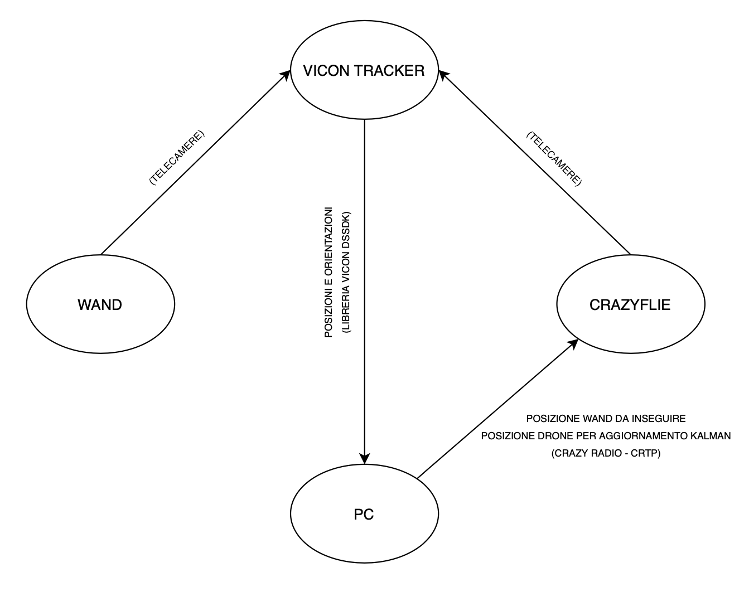
\includegraphics[width=0.8 \textwidth]{Relazione/Immagini/Generale_Progetto.png}
    \caption{Schema a blocchi delle entità coinvolte nel progetto}
    \label{fig:Generale_Progetto}
\end{figure}
\\
\begin{itemize}
    \item Le telecamere, tramite l’individuazione dei marker posizionati sugli oggetti, permettono al Tracker di ricavare in ogni istante posizioni e orientazioni di Drone e Wand;
    \item Tramite le funzioni della libreria Vicon-DSSDK il programma in esecuzione riceve dal tracker le posizioni e le orientazioni di interesse;
    \item Il programma elabora posizioni e orientazioni effettuando eventuali conversioni tra sistemi di riferimento e tramite la Crazyradio e le librerie Python che implementano il protocollo CRTP:
    \begin{itemize}
        \item Fornisce al Drone i nuovi riferimenti di posizione da inseguire, ricavati dalla posizione aggiornata della Wand;
        \item Fornisce al Drone le nuove misure della sua posizione da utilizzare per l’aggiornamento del filtro di Kalman.
    \end{itemize}
    \item E cosi via .. 
\end{itemize}
\\
(più avanti dedicheremo un paragrafo per scendere nel dettaglio di tutte le operazioni necessarie)
